Este capítulo estudia las bases que justifican el diseño de un sistema que utiliza tecnología blockchain para garantizar la integridad, la trazabilidad y la autenticidad de los logs de seguridad. Se analiza la importancia de los logs en los sistemas informáticos y la casuística de aquellos riesgos a los que pueden estar expuestos, en especial, la modificación y/o eliminación de los logs. También se introducen los conceptos más relevantes de la tecnología blockchain y su aplicación en aquellos entornos donde la protección y verificación de los datos es un elemento fundamental.
%%%%%%%%%%%%%%%%%%%%%%%%%%%%%%%%%%%%%%%%%%%%%%%%%%%%%%%%%%%%%%%%%%%%%%%
\subsection{Seguridad Informática}
\subsubsection{Concepto y principios fundamentales}
La seguridad informática se refiere a la protección de los sistemas de información y de sus componentes hardware, software, redes y datos frente a accesos no autorizados, alteraciones, destrucción o divulgación indebida. Esta disciplina ha cobrado relevancia como respuesta al creciente nivel de dependencia de los sistemas digitales y al aumento sostenido de las amenazas cibernéticas. Su objetivo principal es garantizar la confidencialidad, la integridad y la disponibilidad de la información, principios que conforman el modelo conocido como CIA por sus siglas en inglés (Confidentiality, Integrity, Availability)~\cite{Pfleeger2007}.
\begin{itemize}
    \item La confidencialidad significa que la información solo es accesible a aquellos que tienen la autorización correspondiente. Se logra a través de métodos como la criptografía, el control de acceso y la autenticación.
    \item La integridad es la precisión y consistencia de los datos durante el ciclo de vida de la información. Asegúrese a través de la utilización de funciones hash, sumas de comprobación o los logs de auditoría.
    \item La disponibilidad consiste en garantizar que los sistemas informáticos y la información estén accesibles para los usuarios en el momento en que los requieran. Para lograrlo, se implementan mecanismos que permiten mitigar interrupciones en el servicio, como sistemas redundantes, copias de seguridad y planes de recuperación ante desastres~\cite{Stallings2017}.
\end{itemize}
\begin{figure}[H]
    \centering
    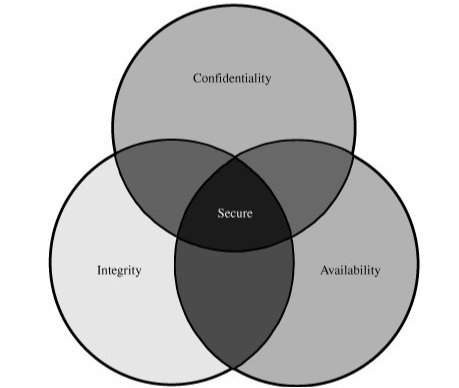
\includegraphics[scale=0.99]{figuras/secure.png}
    \caption{Secure~\cite{Stallings2017}} 
   % \label{fig17}
\end{figure}
A menudo se incorporan otros principios a los tradicionales, como la autenticación, que verifica la identidad de los usuarios; el no repudio, que asegura que una acción o transacción no pueda ser negada por su autor; y la auditoría, que permite rastrear las acciones realizadas dentro del sistema~\cite{Bishop2018}.
Estos principios constituyen la base sobre la cual se diseñan las políticas y mecanismos de seguridad. En el contexto actual, caracterizado por arquitecturas distribuidas, servicios en la nube y tecnologías emergentes como blockchain, la aplicación rigurosa de estos fundamentos resulta esencial para mitigar riesgos y mantener la confianza en los sistemas.

\subsubsection{Amenazas y vulnerabilidades comunes en sistemas de información}
En el ámbito de la seguridad informática, las vulnerabilidades y las amenazas representan los principales riesgos para la integridad, la confidencialidad y la disponibilidad de los sistemas de información. Una amenaza se define como cualquier circunstancia o evento con potencial de causar daño a un sistema o a su información, mientras que una vulnerabilidad corresponde a una debilidad que puede ser explotada por una amenaza para comprometer la seguridad~\cite{Stallings2018}.

Las amenazas se clasifican, en términos generales, en dos categorías: externas e internas. Las amenazas externas provienen de agentes que no forman parte del sistema, como los hackers, el malware, el ransomware, los ataques de denegación de servicio (DDoS) y el phishing. En estos casos, los atacantes suelen aprovechar vulnerabilidades conocidas del software o errores de configuración para infiltrarse en los sistemas~\cite{Pfleeger2007}. Un ejemplo representativo de este tipo de ataques es el ransomware WannaCry, que en 2017 afectó a miles de sistemas a nivel mundial mediante la explotación de una vulnerabilidad en el protocolo SMB de Windows~\cite{Symantec2017}.

Por otro lado, las amenazas internas provienen de usuarios con acceso legítimo a los sistemas, lo que las hace especialmente peligrosas, ya que pueden pasar desapercibidas durante largos periodos. Empleados descontentos, errores humanos o actos negligentes constituyen situaciones comunes asociadas a este tipo de riesgos.

Entre las vulnerabilidades más frecuentes se encuentran las siguientes:
\begin{itemize}
    \item Errores de programación: por ejemplo, desbordamientos de búfer, inyecciones SQL y XSS (cross-site scripting), que permiten ejecutar código malicioso sobre aplicaciones con vulnerabilidades~\cite{OWASP2021}.
    \item Configuraciones incorrectas: servidores mal configurados, puertos abiertos que no deberían estarlo o credenciales por defecto que pueden ser rastreadas y explotadas fácilmente.

    \item Software desactualizado: la falta de actualizaciones y de parches de seguridad incrementan de una forma significativa la posibilidad de explotación de sistemas.

    \item Falta de cifrado de datos: tanto de datos en tránsito como en reposo, la ausencia de cifrado permite hacer volar todo tipo de datos.

    \item Ingeniería social, ataques que manipulan psicológicamente a los usuarios para provocar que faciliten claves o acceso a sistemas.
    
\end{itemize}

La combinación de amenazas y vulnerabilidades dan lugar a los vectores de ataque, es decir, caminos o modos específicos para que un atacante pueda comprometer un sistema. Un ataque típico es enviar un correo de phishing que contiene un enlace a una página falsa (amenaza), aprovechándose de que el usuario no tiene un sistema de verificación multifactor (vulnerabilidad) para robar credenciales de acceso.
En respuesta, las organizaciones deben implantar estrategias proactivas como son auditorías de seguridad, pruebas de penetración, formación continua del personal y políticas estrictas de control de acceso. A partir de este aspecto, es especialmente interesante la utilización de tecnologías emergentes como blockchain para mejorar la trazabilidad y autenticidad de los eventos, lo cual puede suponer una línea de defensa adicional ante modificaciones maliciosas de registros críticos como logs~\cite{Crosby2016}.

\subsubsection{Autenticación, autorización y auditoría}

Los conceptos de autenticación, autorización y auditoría son el fundamento básico para la defensa de los sistemas de información. Con ellos se persigue que los recursos sólo sean utilizados por usuarios válidos y que se pueda registrar las acciones que realiza para su revisión posterior.

La autenticación es la acción a partir de la cual un sistema valida si un usuario o entidad es lo que dice ser. Esto se consigue a través del uso de credenciales clásicas (contraseñas), de tokens, de biometría o de sistemas multifactor, en combinación con al menos dos métodos de verificación~\cite{Stallings2017}.

La autorización, en cambio, se refiere a la posibilidad de poder otorgar permisos a usuarios autenticados y cómo se pueden utilizar los recursos o bien con qué privilegios. Los modelos más utilizados son el control de acceso basado en roles (RBAC) y el control de acceso basado en atributos (ABAC)~\cite{Sandhu1996}.

La auditoría garantiza la obtención, monitorización y análisis de los eventos y actividades del sistema. Su objetivo es detectar comportamientos irregularidad, buscar ataques y permitir la trazabilidad. Un sistema de auditoría óptimo es necesario para el cumplimiento de las normas de seguridad y para la reconstrucción de los incidentes tras una brecha~\cite{Bishop2018}.

Cuando se aplican adecuadamente estos tres mecanismos suponen una importante capa defensiva de cualquier infraestructura tecnológica contemporánea.


%%%%%%%%%%%%%%%%%%%%%%%%%%%%%%%%%%%%%%%%%%%%%%%%%%%%%%%%%%%%%%%%%
\subsection{Blockchain}
\subsubsection{ Origen y evolución del blockchain}
La idea de blockchain aparece como una forma de poder registrar las transacciones de forma segura, descentralizada y resistente a la manipulación. Esta idea toma su origen en el artículo que publicó el conocido pseudónimo de Satoshi Nakamoto en 2008 con el que se propuso una moneda digital, el Bitcoin, que estaba estructurada sobre una forma de datos encadenados cronológicamente de la que se hablaba como de cadena de bloques~\cite{nakamoto2008bitcoin}, lo cual servía para poder registrar transacciones entre pares sin la necesidad de tener un ente central que se hiciera cargo de ello y permitía así resolver el problema de los dobles gastos en entornos digitales.
A pesar de que el término “blockchain” suena en relación a Bitcoin, su antecedente teórico se remonta a décadas pasadas, en 1991 Stuart Haber y W. Scott Stornetta proponían un método mediante el cual se pudiera certificar la inmutabilidad de los documentos digitales recurriendo a un sistema de sellado de tiempo que fuera criptográfico~\cite{Haber1991}. Posteriormente, en el año 1997, las partes interesadas introdujeron el concepto de árboles de Merkle, que permiten verificar conjuntos de datos muy grandes con una mayor eficiencia.
La historia del blockchain ha acometido distintas etapas relevantes. En primer lugar, la primera generación de blockchain, representada por Bitcoin, introdujo transacciones financieras completamente descentralizadas. Esta implementación demostró la capacidad de mantener registros inmutables sin depender de un intermediario de confianza; no obstante, su funcionalidad se limitaba a operaciones predefinidas.~\cite{nakamoto2008bitcoin}.

\begin{figure}[h!]
\centering
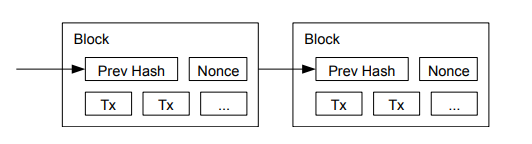
\includegraphics[width=0.7\textwidth]{figuras/blockchain.png} 
\caption{Estructura básica de una blockchain \cite{nakamoto2008bitcoin}}
\label{fig:blockchain_estructura}
\end{figure}
La Figura~\ref{fig:blockchain_estructura} ilustra la estructura fundamental de una blockchain, tal como fue concebida originalmente~\cite{nakamoto2008bitcoin}. Cada bloque contiene un puntero al hash del bloque anterior denominado \textit{“Prev Hash”} lo que garantiza la continuidad y el orden dentro de la cadena. Además, incorpora un conjunto de transacciones (Tx) que han sido validadas y añadidas al registro. El campo “Nonce” es un número aleatorio que los mineros modifican durante el proceso de Proof of Work hasta encontrar un hash que cumpla con los criterios establecidos por la red. Una vez se encuentra un hash válido, este se incluye en el bloque y, posteriormente, se incorpora como referencia en el siguiente bloque, conformando así una cadena inalterable y resistente a manipulaciones.

Tras ello, en 2015, con la llegada de Ethereum comenzó la segunda generación de blockchain, que permitió la creación de los smart contracts, programas que se ejecutan automáticamente, se almacenan en la cadena de bloques y se activan siempre que se cumplan ciertas condiciones~\cite{Buterin2014}. Esta innovación amplió enormemente las aplicaciones de la blockchain, incluyendo la automatización de procesos jurídicos, financieros o logísticos, entre otros.

Actualmente, se habla de una tercera generación de blockchain, representada por plataformas como Cardano, Polkadot o Algorand, que intentan solucionar los problemas de escalabilidad, interoperabilidad y eficiencia energética a medida que buscan no sacrificar la descentralización ni la seguridad~\cite{Swan2015}. Estas plataformas emplean algoritmos de consenso más sofisticados, como Proof of Stake (PoS) o Byzantine Fault Tolerance (BFT), en contraposición al intensivo mecanismo Proof of Work (PoW) de Bitcoin.

Además, han surgido distintos tipos de blockchain según su nivel de acceso y gobernanza: públicas (abiertas y descentralizadas), privadas (exclusivas para ciertos entes) y consorciadas (autogestionadas por un grupo de organizaciones)~\cite{Xu2017}. La diversidad de estas plataformas ha facilitado su adopción en ámbitos como la salud, la educación, la logística y, de forma destacada, la ciberseguridad, donde se utilizan para mejorar la trazabilidad e integridad de la información, por ejemplo en los logs de seguridad.

La blockchain ha evolucionado de ser una solución financiera descentralizada a convertirse en un marco versátil con aplicaciones transversales en múltiples sectores. Su crecimiento ha acompañado tanto el avance tecnológico como la demanda de sistemas confiables, transparentes e inmutables en entornos donde la integridad de los datos resulta crítica.

\subsubsection{ Arquitectura de blockchain (bloques, cadena, nodos)}
La arquitectura de una blockchain se basa en una estructura de datos distribuida especialmente diseñada para el registro inmutable de transacciones. Esta arquitectura está compuesta fundamentalmente por bloques, que se enlazan de forma secuencial formando una cadena, y por una red de nodos que participan en el mantenimiento y la validación de dicha cadena.

Cada bloque contiene un conjunto de transacciones agrupadas junto con información adicional, generalmente denominada metadatos. Entre estos metadatos se incluyen el hash del bloque anterior, la marca de tiempo (fecha y hora), y en blockchains basadas en el mecanismo de Proof of Work, un valor denominado nonce (un número aleatorio que los mineros modifican para encontrar un hash válido). Estos elementos permiten garantizar la integridad y seguridad de la cadena. 

El encabezado de un bloque no solo incluye el hash del bloque anterior, la marca de tiempo y el nonce, sino también un resumen hash de todas las transacciones, generalmente mediante un árbol de Merkle. Esto permite verificar de forma eficiente la integridad individual de las transacciones, sin necesidad de revisar todo el contenido del bloque~\cite{Stallings2017}. Esta organización se encarga de garantizar que cualquier alteración a los datos de un bloque altere su respectivo hash, quebrando la conexión con el siguiente bloque y, como consecuencia, el hecho de que los datos han sido alterados.

La cadena de bloques es el resultado del enlazado criptográfico y en orden temporal de los bloques. Esta función de encadenar los bloques mediante hashes permite asegurar la inmutabilidad del historial de transacciones, ya que se requiere rehacer todos los hashes de los bloques posteriores al que haya sido alterado y, además, obtener el consenso de la red, lo cual resulta computacionalmente inviable en blockchains públicas con mecanismos como Proof of Work o Proof of Stake~\cite{nakamoto2008bitcoin}.

Los nodos son las entidades que actúan dentro de la red blockchain. El tipo de nodo y el tipo de blockchain determinan las funciones que puede desempeñar. Así, existen nodos que solo almacenan copias del libro mayor (nodos ligeros) y otros que participan activamente en el consenso, validando transacciones y agregando bloques al libro mayor (nodos validadores o mineros)\cite{Swan2015}. Del mismo modo, en redes como Hyperledger Fabric, los nodos tienen roles específicos: peers, que almacenan los libros mayores y ejecutan smart contracts; orderers, que garantizan el orden de las transacciones; o clients, que inician las solicitudes\cite{HyperledgerFabric2.5KeyConcepts}.

En el caso de blockchains permisadas como Hyperledger Fabric, la arquitectura de red permite una mayor modularidad y control sobre quién puede actuar como nodo y qué operaciones puede realizar. A diferencia de las cadenas públicas, donde cualquier usuario puede convertirse en nodo, en las blockchains empresariales se aplican políticas de acceso basadas en identidades verificadas y certificados digitales~\cite{HyperledgerFabric2.5KeyConcepts}. Por lo tanto, toda interacción entre bloques, la cadena criptográfica y los nodos participantes se realiza en un entorno de confianza sin intermediarios. Este tipo de arquitectura es ideal para casos en los que se requiere garantizar integridad y trazabilidad, como en la gestión de logs de seguridad.



\subsubsection{Propiedades principales: inmutabilidad, descentralización, transparencia}

Las características más importantes que permiten la diferenciación de blockchain son la inmutabilidad, la descentralización y la transparencia, presentando las bases garantizadoras de su fiabilidad y de la posibilidad de aplicarse en entornos donde la seguridad y la trazabilidad son las premisas a cumplir.

La inmutabilidad hace referencia a que, cuando los datos están ya registrados en la cadena de blocks, parezca prácticamente imposible su modificación. Tal característica se garantiza por medios de técnicas criptográficas como son las funciones hash y la estructura de encadenado de los blocks. Esto permite que cualquier tentativa de modificación sea identificada fácilmente~\cite{Stallings2017}.

La descentralización, por el contrario, no requiere de una entidad central a la que se le pueda dar confianza. Más bien, una vez más, la validación y almacenamiento de la información se distribuyen y llevan a cabo por muchos nodos que forman parte de la red. Como resultado, el aumento en la tolerancia a errores se verá ocultado de igual manera por la disminución de posibilidades de censura o manipulación de la información~\cite{nakamoto2008bitcoin}.

La transparencia lleva a los participantes afines a poder comprobar el estado y la historia de las transacciones, incrementando la posibilidad de confianza en un sistema colaborativo. La visibilidad será variable según sea el tipo de blockchain que incluyamos (público o privado), pero la certeza de la trazabilidad de los hechos sometidos a verificación será constante~\cite{Crosby2016}.
Estas características hacen que blockchain pueda considerarse como un elemento adecuado para poder asegurar la integridad y autenticidad de la información sensible como podrían ser el caso de los logs de seguridad.

\subsubsection{Funciones hash y su importancia en blockchain}
Las funciones hash criptográficas constituyen uno de los pilares fundamentales de la tecnología blockchain, ya que permiten transformar una entrada de datos de cualquier longitud en una salida de longitud fija, denominada hash o digest. Esta salida es única para cada entrada diferente, de modo que incluso una mínima alteración en los datos originales genera un hash completamente distinto~\cite{bishop2003computer}.

En el contexto de blockchain, las funciones hash cumplen múltiples roles esenciales. El más importante de ellos es garantizar la integridad de los datos. Cada bloque en la cadena contiene el hash del bloque anterior, lo que establece una dependencia secuencial entre los bloques. Esta estructura implica que cualquier modificación en un bloque altera su hash, rompiendo así la continuidad de la cadena y haciendo evidente la manipulación~\cite{axelsson2000ids}.

Esta propiedad ofrece una defensa efectiva frente a intentos de alteración o falsificación de los datos.
Otra función destacada de los algoritmos hash en blockchain es la verificación eficiente de la información. Como el hash actúa como una firma digital del contenido, los nodos pueden validar la autenticidad de los datos sin necesidad de revisar su totalidad. Esto reduce significativamente la carga computacional y mejora el rendimiento general del sistema~\cite{iso27001}.

Además, las funciones hash desempeñan un papel clave en los mecanismos de consenso, como el Proof of Work (PoW), utilizado en la blockchain de Bitcoin. En este esquema, los mineros deben encontrar un valor denominado nonce que, al ser combinado con los datos del bloque, genere un hash que cumpla con ciertas condiciones predefinidas, como comenzar con un número específico de ceros. Este proceso, conocido como minería, es computacionalmente costoso y aleatorio, pero su verificación es sencilla, lo que asegura que la incorporación de nuevos bloques requiera un esfuerzo considerable y dificulta ataques como el double spend~\cite{kabiri2005survey}.

Las funciones hash también se utilizan en estructuras de datos como los árboles de Merkle, que permiten comprobar si una transacción está incluida en un bloque sin necesidad de descargar el bloque completo. Esto reduce el uso de ancho de banda y almacenamiento, una ventaja crucial especialmente en dispositivos con recursos limitados~\cite{kent2006log}.

Para cumplir adecuadamente su rol en blockchain, las funciones hash deben presentar ciertas propiedades criptográficas fundamentales: resistencia a colisiones, resistencia a la preimagen y resistencia a la segunda preimagen. Estas propiedades aseguran que no puedan encontrarse dos entradas distintas con el mismo hash, ni reconstruir la entrada original a partir del hash, garantizando así la seguridad del sistema~\cite{axelsson2000base}.
\subsubsection{ Firmas digitales y autenticación}
Las firmas digitales constituyen un componente fundamental en la infraestructura de seguridad de los sistemas blockchain, ya que permiten garantizar tanto la autenticación como la integridad de los datos. Estas firmas se basan en algoritmos criptográficos de clave pública, mediante los cuales el emisor firma un mensaje con su clave privada, y el receptor puede verificar su autenticidad utilizando la clave pública correspondiente~\cite{stallings2017crypto}.

En las plataformas blockchain, cada transacción es firmada digitalmente por su emisor, lo que asegura que proviene de un usuario legítimo y que no ha sido alterada durante su transmisión en la red. Este mecanismo permite mantener un entorno seguro sin la necesidad de una autoridad central~\cite{nakamoto2008bitcoin}.

Uno de los algoritmos más utilizados para este propósito es el Elliptic Curve Digital Signature Algorithm (ECDSA), conocido por su eficiencia y por ofrecer un alto nivel de seguridad incluso utilizando claves más cortas que las empleadas por RSA~\cite{Koblitz2004}.

La autenticación en blockchain se basa en el uso de criptografía de clave pública. Cada participante posee un par de claves (pública y privada), lo que permite identificar de forma única a cada nodo o usuario del sistema. Este enfoque elimina la necesidad de contraseñas o intermediarios, mejorando la seguridad y la escalabilidad de la red~\cite{Bishop2019}.

En redes como Hyperledger Fabric, las firmas digitales y la autenticación se gestionan mediante certificados digitales emitidos por una Autoridad Certificadora (CA), conforme al estándar X.509~\cite{HyperledgerFabric2.5Identity}.

\subsubsection{Criptografía de clave pública y privada}
La criptografía de clave pública y privada, también conocida como criptografía asimétrica, es uno de los componentes fundamentales de los sistemas de seguridad actuales y, en particular, de la tecnología blockchain. A diferencia de la criptografía simétrica, que emplea una única clave tanto para el cifrado como para el descifrado de los datos, la criptografía asimétrica se basa en un par de claves. La clave pública puede compartirse abiertamente, mientras que la clave privada debe mantenerse en secreto~\cite{Stallings2017}.

Este mecanismo permite implementar funciones esenciales como la autenticación, la confidencialidad, la integridad y el no repudio. En los sistemas blockchain, las claves públicas se utilizan para identificar a los usuarios, mientras que las claves privadas permiten generar firmas digitales que validan las transacciones. Solo el titular legítimo de la clave privada puede producir una firma considerada válida, lo cual asegura que las transacciones provienen de un usuario autorizado y que pueden verificarse mediante la clave pública correspondiente~\cite{Bishop2019}.

Entre los algoritmos más utilizados en este tipo de criptografía se encuentran RSA, desarrollado por Rivest, Shamir y Adleman, y ECDSA, conocido como el algoritmo de firma digital basado en curvas elípticas. Aunque RSA ha sido históricamente el estándar más empleado, ECDSA ha cobrado mayor relevancia en aplicaciones blockchain debido a su mayor eficiencia y a su capacidad de ofrecer el mismo nivel de seguridad con claves de menor longitud~\cite{Koblitz2004}.

La criptografía de clave pública también permite la utilización de certificados digitales en infraestructuras como Hyperledger Fabric. En este tipo de redes, una Autoridad Certificadora valida la identidad de los participantes conforme al estándar X.509~\cite{HyperledgerFabric2.5Identity}.

\subsubsection{Tipos de blockchain: pública, privada y consorciada}
Los sistemas de blockchain pueden clasificarse fundamentalmente en tres tipos: públicos, privados y consorciados, diferenciándose por sus restricciones de acceso a la red, así como por los mecanismos de control y gobernanza para los miembros de la misma~\cite{Tapscott2016}.

Una blockchain pública se caracteriza por permitir que cualquier persona o entidad se una a la red, visualice las transacciones y participe en el proceso de consenso sin requerir permisos explícitos. Bitcoin y Ethereum son ejemplos típicos. Aunque ofrecen altos niveles de descentralización y transparencia, suelen presentar problemas de rendimiento transaccional y elevado consumo de recursos, especialmente en redes que utilizan Proof of Work~\cite{Antonopoulos2017}.

Por el contrario, una blockchain privada está bajo el control de una única organización, la cual define quién puede acceder a la red y quién valida las transacciones. Este modelo es adoptado con frecuencia por entidades que buscan un mayor grado de privacidad, seguridad y eficiencia para cumplir su misión empresarial. Aunque reduce la descentralización, las blockchains privadas permiten un control más estricto sobre los datos y el rendimiento de la red~\cite{Lee2011}.

Las blockchains consorciadas, también llamadas federadas, combinan características de los dos modelos anteriores. Son gestionadas por un grupo de organizaciones previamente seleccionadas, que comparten la responsabilidad de administrar la red y validar las transacciones. Este enfoque es especialmente útil y preferido en sectores donde múltiples entidades necesitan colaborar manteniendo cierto grado de confianza y control, como en el ámbito financiero o en la gestión de cadenas de suministro~\cite{Wood2014}.
\subsubsection{Smart contracts y Chaincode}
Los smart contracts, o contratos inteligentes, pueden definirse o bien como los programas que se ejecutan de manera automática cuando se cumplen ciertas condiciones previamente definidas, dejando de lado a los intermediarios y permitiendo así el cumplimiento de los contratos~\cite{Swan2015} o como el concepto que publicó Nick Szabo en 1994, quien los define como protocolos de transacciones digitales que ejecutan automáticamente los términos de un contrato~\cite{Szabo1996}-.
En cada plataforma, cada blockchain, los smart contracts se encuentran escritos en lenguajes específicos por ejemplo, en el caso de Ethereum el lenguaje de programación es Solidity y se despliegan en la blockchain pública, por lo que también otorgan transparencia, inmutabilidad y accesibilidad~\cite{EthereumWhitePaper}.

Mediante los smart contracts, se pueden desarrollar aplicaciones descentralizadas, conocidas como DApps, para fines muy diversos, desde las finanzas hasta la gestión de identidad.

En el mundo empresarial, Hyperledger Fabric introduce el término Chaincode como el equivalente al smart contract. El Chaincode puede entenderse como un programa que define la lógica de negocio que se ejecuta en el entorno de Fabric. A diferencia de Ethereum, Fabric permite el despliegue de contratos en canales públicos o restringidos, donde el uso de la blockchain requiere control por parte de las organizaciones participantes, lo que permite mayor privacidad y manejo de datos~\cite{HyperledgerFabricChaincode}.

Del mismo modo, Fabric permite escribir y desplegar contratos en otros lenguajes de programación, como Go y JavaScript, entre otros, facilitando así la integración de smart contracts dentro de un entorno corporativo. Estos contratos pueden desplegarse en canales tanto públicos como privados, ampliando con ello las posibilidades de uso de blockchain según el nivel de privacidad y escalabilidad.
%%%%%%%%%%%%%%%%%%%%%%%%%%%%
\subsection{Tecnologías blockchain existentes}
A fin de ilustrar mejor las diferencias entre algunas de las tecnologías blockchain más utilizadas, se presenta una comparación en la Tabla~\ref{tab:comparacion_blockchains}. En ella se destacan aspectos como el tipo de red, el algoritmo de consenso, el soporte para smart contracts, y los principales casos de uso. Esta información resulta útil para contextualizar la evolución de estas plataformas y su adecuación a distintos entornos, tanto públicos como empresariales.

\newpage
\begin{table}[h!]
\centering
\captionsetup{list=no} % Esto evita que se añada automáticamente al índice
\caption{COMPARACIÓN DE TECNOLOGÍAS BLOCKCHAIN}
\addcontentsline{lot}{table}{Tabla \thetable. Comparación de tecnologías blockchain}
\label{tab:comparacion_blockchains}
\begin{tabularx}{\textwidth}{l l l X}
\toprule
\textbf{Tecnología} & \textbf{Tipo} & \textbf{Consenso} & \textbf{Características principales} \\
\midrule
Bitcoin & Pública & Proof of Work (PoW) & Enfocada en transferencias de valor \cite{Narayanan2016} \\
Ethereum & Pública & Proof of Stake (PoS) & Smart contracts y DApps \cite{EthereumWhitePaper} \\
Hyperledger Fabric & Permisionada & Pluggable (Raft, etc.) & Modular, privada, orientada a empresas \cite{HyperledgerFabric} \\
Corda & Permisionada & Notary Nodes & Privacidad punto a punto, orientado a finanzas \cite{R3Corda2021} \\
\bottomrule
\end{tabularx}
\end{table}

\subsubsection{Bitcoin}
Bitcoin, la primera criptomoneda, fue publicada en 2008 por una persona o un grupo de personas con el pseudónimo Satoshi Nakamoto \cite{nakamoto2008bitcoin}, y al mismo tiempo representa la primera implementación exitosa de una blockchain pública y descentralizada. Bitcoin se basa en un libro de contabilidad que es distribuido y transparente, en el cual las transacciones se agrupan en bloques y se encadenan criptográficamente, lo cual garantiza la inmutabilidad e integridad de los datos \cite{Antonopoulos2014}. El mecanismo de consenso subyacente es \textit{Proof of Work} (PoW), que requiere que los participantes de la red (mineros) resuelvan complejos problemas computacionales para validar y añadir nuevos bloques a la cadena. Este proceso no solo asegura la red contra ataques, sino que también incentiva la participación a través de la recompensa en nuevos bitcoins y tarifas de transacción \cite{Narayanan2016}.

La arquitectura de Bitcoin se puede analizar en varios niveles interconectados que permiten su funcionamiento como un sistema de efectivo electrónico descentralizado y resistente a la censura. Estos niveles incluyen la red \textit{peer-to-peer}, la blockchain en sí misma, las transacciones y el mecanismo de consenso. Bitcoin opera sobre una red distribuida de nodos (ordenadores que ejecutan el software de Bitcoin). No existe un servidor central; en cambio, cada nodo mantiene una copia de la blockchain (completa o podada) y participa en la validación y retransmisión de transacciones. Cuando un usuario inicia una transacción, esta se difunde a los nodos vecinos, propagándose por toda la red hasta que alcanza a la mayoría de los participantes. Esta naturaleza distribuida es fundamental para la descentralización y la resistencia a puntos únicos de fallo \cite{Swan2015}.

La blockchain constituye el corazón de Bitcoin. Se trata de un registro público, secuencial y cronológico de todas las transacciones de Bitcoin que se han realizado. Los datos constan en bloques, los cuales agrupan un conjunto de transacciones autenticadas, hacen referencia al bloque anterior (a través de un hash criptográfico), hacen constar una marca de tiempo y contienen un \textit{nonce} (número que se utiliza una sola vez) que se ha utilizado en el proceso de \textit{Proof of Work}. La cadena criptográfica existente entre los bloques garantiza que cualquier modificación en un bloque anterior provocaría la invalidez de todos los bloques posteriores, asegurando de este modo la inmutabilidad del registro \cite{drescher2017blockchain}.

Una transacción de Bitcoin toma la forma de una transferencia de valor entre direcciones (identificadores alfanuméricos resultantes de claves públicas), de tal forma que cada transacción incluye una o más “entradas” (referencias a bitcoins que han pasado a estar disponibles para ser gastados) y una o varias “salidas” (especifican las nuevas direcciones de destino y la cantidad de bitcoins que se desea transferir). Para evitar el doble gasto, las transacciones deben ser confirmadas (o, si se quiere, validadas) por la red mediante el proceso de minería e incluidas en un bloque. Las transacciones se firman de manera digital mediante la clave privada del remitente, lo cual, en este caso, representa la propiedad de los bitcoins que se quieren mover \cite{Antonopoulos2014}.

Para lograr que todos los nodos de la red de Bitcoin lleguen a un acuerdo sobre la historia de las transacciones y para evitar comportamientos maliciosos, se utiliza el algoritmo de consenso denominado \textit{Proof of Work} (PoW). En este algoritmo, los mineros compiten contra el resto de mineros en la tarea de encontrar la solución para un complejo problema criptográfico a la hora de proponer un bloque. El primer minero en encontrar una solución válida (un \textit{nonce} que, junto con la información del bloque y la aplicación de una función hash, produzca un hash que cumpla con un cierto nivel de dificultad) tiene ahora la opción de agregar el bloque a la blockchain. Este proceso requiere una elevada cantidad de potencia de cómputo y energía, lo que hace que sea costoso y, por ende, disuasorio para perpetrar ataques \cite{Buterin2014}. El bloque validado se propaga a través de la red y el resto de nodos lo verifican e incluyen en su propia copia de la blockchain.

\subsubsection{Ethereum}
Ethereum, propuesto por Vitalik Buterin en 2013 y lanzado en 2015, es una plataforma blockchain de código abierto que va más allá de la simple transferencia de valor, introduciendo la funcionalidad de smart contracts y aplicaciones descentralizadas (DApps) \cite{EthereumWhitePaper}. Su objetivo principal es permitir a los desarrolladores construir y desplegar aplicaciones que se ejecuten sobre una infraestructura descentralizada y segura, sin la necesidad de intermediarios. Ethereum se distingue de Bitcoin por su lenguaje de programación Turing-completo, Solidity, que permite la creación de lógica de negocio compleja dentro de los smart contracts \cite{Wood2014}.

La arquitectura de Ethereum comparte similitudes con Bitcoin en cuanto a su naturaleza descentralizada y el uso de una blockchain para registrar transacciones. Sin embargo, presenta diferencias significativas en su mecanismo de consenso y en la finalidad de su diseño. Inicialmente, Ethereum utilizaba el algoritmo de consenso Proof of Work (PoW) al igual que Bitcoin, pero realizó una transición significativa a Proof of Stake (PoS) con la actualización The Merge en 2022. En PoS, los validadores son seleccionados para proponer y verificar nuevos bloques basándose en la cantidad de Ether (la criptomoneda nativa de Ethereum) que han apostado o bloqueado como garantía \cite{Buterin2014}. Este cambio se realizó con el objetivo de mejorar la eficiencia energética y la seguridad de la red.

La blockchain de Ethereum también se organiza en bloques enlazados criptográficamente, asegurando la inmutabilidad de los datos. Cada bloque contiene un hash del bloque anterior, un timestamp y un conjunto de transacciones. Sin embargo, a diferencia de Bitcoin, los bloques de Ethereum también contienen el estado actual de la máquina virtual de Ethereum (EVM), el entorno de ejecución para los smart contracts. Cada transacción en Ethereum puede ser una simple transferencia de Ether o la ejecución de un smart contract, lo que implica la modificación del estado de la EVM \cite{EthereumYellowPaper}.

Los smart contracts son programas de código que se ejecutan en la EVM y se almacenan en la blockchain de Ethereum. Estos contratos pueden definir reglas para la transferencia de activos digitales, la creación de organizaciones autónomas descentralizadas (DAOs), la implementación de mercados descentralizados (DEXs) y muchas otras aplicaciones. Una vez desplegado, un contrato inteligente es inmutable y se ejecuta de manera autónoma cuando se cumplen las condiciones definidas en su código \cite{Szabo1997}.

La red \textit{peer-to-peer} de Ethereum está compuesta por nodos que ejecutan diferentes implementaciones del cliente de Ethereum. Estos nodos participan en la propagación de transacciones y bloques, así como en la verificación del estado de la blockchain y la ejecución de los smart contracts. La transición a PoS también introdujo el concepto de nodos validadores, que son responsables de proponer y atestiguar nuevos bloques, reemplazando el rol de los mineros en el sistema PoW anterior.

\subsubsection{Hyperledger Fabric}
Hyperledger Fabric es una plataforma de blockchain de código abierto, desarrollada bajo el paraguas de la Hyperledger Foundation, que se enfoca en casos de uso empresarial. A diferencia de blockchains públicas y sin permisos como Bitcoin y Ethereum, Hyperledger Fabric es una blockchain permisionada, lo que significa que los participantes deben tener una identidad conocida y autorizada para interactuar con la red \cite{HyperledgerFabric}. Esta característica la hace especialmente adecuada para aplicaciones empresariales donde la privacidad, la confidencialidad y el cumplimiento normativo son requisitos cruciales.

\begin{figure}[htb]
\centering
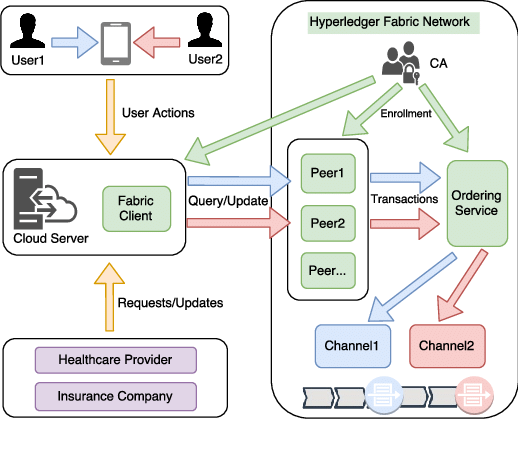
\includegraphics[width=0.7\textwidth]{figuras/hyperledger_fabric_architecture.png}
\caption{Arquitectura de Hyperledger Fabric mostrando la interacción entre usuarios \cite{RadwHyperledger2018}}
\label{figura:hyperledger_architecture}
\end{figure}

La arquitectura de Hyperledger Fabric, como se muestra en la Figura \ref{figura:hyperledger_architecture}, se distingue por su diseño modular y flexible. Permite a las empresas construir redes blockchain privadas o consorciadas adaptadas a sus necesidades específicas. Uno de los componentes clave de Fabric es el concepto de “canales”, que proporcionan carriles de comunicación privados y confidenciales para subconjuntos de la red. Esto asegura que la información sensible solo sea compartida entre las partes autorizadas \cite{Androulaki2018}.

El mecanismo de consenso en Hyperledger Fabric es \textit{pluggable}, lo que significa que diferentes algoritmos de consenso pueden ser implementados y configurados según los requisitos de la aplicación. Algunos de los mecanismos de consenso admitidos incluyen Raft , Kafka (un sistema de mensajería distribuido, utilizado para el ordenamiento de transacciones) y, en el futuro, otros algoritmos tolerantes a fallos bizantinos (BFT) para una mayor robustez en entornos con participantes potencialmente maliciosos \cite{Cachin2011}. La elección del mecanismo de consenso depende de los requisitos de confianza y rendimiento de la red.

Otro componente fundamental de Hyperledger Fabric son los \textit{chaincodes}, que son equivalentes a los smart contracts en otras plataformas blockchain. Los \textit{chaincodes} son programas de código (escritos en lenguajes como Go, Java y Node.js) que definen la lógica de negocio y las reglas para interactuar con el libro mayor (\textit{ledger}) de la blockchain. Los \textit{chaincodes} se instalan, instancian y ejecutan en nodos específicos de la red, y su ejecución genera transacciones que se registran en la blockchain \cite{HyperledgerFabricDocs}.

La gestión de la identidad es otro aspecto crucial de Hyperledger Fabric. Utiliza un servicio de pertenencia (Membership Service Provider - MSP) para gestionar las identidades de los participantes, los roles y los permisos dentro de la red. Esto asegura que solo las entidades autorizadas puedan acceder a la red y realizar transacciones \cite{HyperledgerFabricMSP}.

\subsubsection{Corda}
Corda es una plataforma de blockchain de código abierto diseñada específicamente para las necesidades de las empresas reguladas, particularmente en el sector financiero. A diferencia de otras plataformas blockchain que buscan replicar datos a través de una red amplia, Corda adopta un enfoque de consenso restringido y privacidad punto a punto. Esto significa que los datos de las transacciones solo se comparten con las partes directamente involucradas en esa transacción y con los nodos notarios que validan la singularidad de las transacciones, evitando el doble gasto \cite{R3Corda2021}.

La arquitectura de Corda se centra en la eliminación de la necesidad de una replicación global de datos, lo que puede mejorar significativamente la privacidad y la escalabilidad en entornos empresariales. Las transacciones en Corda se representan como “estados”, que son objetos inmutables registrados en el ledger. Estos estados pueden representar acuerdos legales, instrumentos financieros u otros tipos de activos digitales. Las transacciones proponen transiciones entre estos estados, y para que una transacción sea válida, debe ser firmada por las partes necesarias y validada por uno o más nodos notarios \cite{Hearn2016}.

El mecanismo de consenso en Corda se basa en los nodos notarios. Estos nodos no mantienen una copia completa de toda la blockchain, sino que actúan como terceros de confianza que verifican que las transacciones no involucran entradas (estados) que ya han sido consumidas en otra transacción. Diferentes tipos de notarios pueden ser implementados, ofreciendo distintos niveles de tolerancia a fallos y rendimiento \cite{Brown2018}. La elección del notario es fundamental para la confianza y la finalidad de las transacciones en la red Corda.

Los “CorDapps” (Corda Distributed Applications) son el equivalente a las aplicaciones descentralizadas en otras plataformas. Son paquetes de código (escritos principalmente en Kotlin o Java) que definen los flujos de trabajo de negocio, las estructuras de los estados y los contratos (la lógica que rige la evolución de los estados). Los CorDapps permiten a las empresas construir aplicaciones blockchain interoperables que pueden interactuar con otras partes en la red Corda dentro del contexto de acuerdos específicos \cite{R3CordaDocs}.

La estructura del ledger en Corda es una colección de estados inmutables. Cada participante en la red mantiene una bóveda (vault) que contiene los estados relevantes para ellos. Cuando se realiza una transacción, solo las partes involucradas ven los detalles de esa transacción registrada en sus respectivas bóvedas. Esto contrasta con las blockchains públicas donde todas las transacciones son visibles para todos los participantes. La privacidad se refuerza mediante el uso de claves criptográficas y la limitación de la distribución de datos \cite{R3CordaPrivacy}.

La gestión de la identidad en Corda se basa en un servicio de directorio que asigna identidades del mundo real a claves criptográficas. Esto permite a las partes saber con quién están interactuando en la red. La identidad es fundamental para establecer acuerdos legales y responsabilidades en un entorno empresarial regulado \cite{R3CordaIdentity}.



Estas tecnologías se adaptan a distintos contextos según los requerimientos de privacidad, escalabilidad y gobernanza del sistema.


%%%%%%%%%%%%%%%%%%%%%%%%%%%%%%%%%%%%%%%%%%%%%%%%%%%%%%%%%%%%%%%%
\subsection{Logs}
\subsubsection{Definición y función de los logs de seguridad}
Los logs de seguridad son la representación gráfica y temporal de la seguridad de un sistema informático o de una red de ordenadores. En resumen, un log de seguridad es el registro de actividades que podrían afectar la integridad, disponibilidad y confidencialidad de los recursos tecnológicos. En el contexto de la seguridad informática, un log puede contener información sobre accesos, intentos de autenticación, modificaciones de ficheros, cambios en la configuración del sistema y eventos de los dispositivos de seguridad como los firewalls, los sistemas de detección de intrusos (IDS) o los antivirus~\cite{bishop2003computer}.

La principal finalidad de los logs de seguridad es proporcionar la información adecuada para la monitorización, la auditoría y el análisis de incidentes de seguridad. A través de los logs, los administradores de sistemas y los equipos de respuesta a incidentes pueden reconstruir la serie de acontecimientos que culminaron en un posible incidente. Esto permite identificar las vulnerabilidades que han sido objetivo de ataque, las acciones llevadas a cabo por los atacantes y el impacto del evento~\cite{Landauer2020}. Además, los logs permiten comprobar la integridad del sistema y si las políticas de seguridad están siendo cumplidas.

Una definición formal de logs de seguridad se puede encontrar en los libros, donde se consideran como “documentos electrónicos en los que se recogen las actividades que se desarrollan en un sistema de información, permitiendo la trazabilidad y el análisis forense de los sucesos”~\cite{Landauer2020}.

\subsubsection{Importancia de los logs en la gestión de la seguridad informática}
En el marco de la seguridad de la información, los logs constituyen una fuente esencial de prueba para la recogida de evidencias, auditoría, detección de amenazas y análisis forense. Su importancia reside en que permiten registrar de forma ordenada a través del tiempo las actividades que tienen lugar en los sistemas de información, constituyendo una base firme para la identificación de comportamientos anómalos, atribución de ataques, y verificación de que se cumple con las políticas de seguridad predefinida~\cite{bishop2003computer}.

Los logs son determinantes para garantizar el seguimiento y trazabilidad de las actividades, por usuarios o sistemas; esta trazabilidad es fundamental para la investigación de los incidentes, dado que permite la reconstrucción de la secuencia de eventos que condujeron a la explotación de una vulnerabilidad o a una violación de la seguridad~\cite{axelsson2000ids}. En muchas normativa y estándares internacionales (ISO/IEC 27001, NIST SP 800-53) se indica explícitamente la necesidad de implementar un mecanismo de registro y auditoría con el fin de mejorar la postura de seguridad de las organizaciones~\cite{iso27001}.

Otra de las funciones determinantes de los logs es su capacidad para detectar las amenazas en fase temprana. Sistemas automáticos como los SIEM (Seguridad, información y gestión de eventos) son sistemas que recogen, normalizan y analizan grandes volúmenes de registros con el objetivo de detectar patrones sospechosos que pueden pasar desapercibidos en la revisión manual. Estos sistemas pueden emitir alertas en tiempo real y permitir una respuesta rápida ante incidentes potenciales, minimizando así el daño ~\cite{kabiri2005survey}.

\subsubsection{Retos y problemas comunes en la gestión de logs (manipulación, pérdida, falsificación)}
La administración de logs de seguridad es un aspecto fundamental en cualquier política de ciberprotección adoptada por las organizaciones. Sin embargo, su implementación y gestión enfrentan diversas dificultades operativas y técnicas, tales como la manipulación maliciosa, la pérdida accidental o intencionada, y la falsificación de registros. Estos problemas ponen en entredicho la validez de los logs y, por ende, la eficacia de los procesos de auditoría, análisis forense y respuesta a incidentes~\cite{kent2006log}.

Uno de los principales desafíos es la manipulación de logs. Los atacantes que obtienen acceso a sistemas privilegiados alteran registros para ocultar sus huellas y evitar ser detectados. Esta manipulación puede manifestarse mediante la modificación de las marcas de tiempo, la eliminación de eventos relevantes o la introducción de registros falsos que confunden a los analistas de seguridad~\cite{axelsson2000base}.

Dicha alteración compromete la integridad del sistema de logs, dificulta la reconstrucción de los eventos y puede impedir que las organizaciones comprendan la verdadera naturaleza de una violación de seguridad.

Otro problema significativo es la pérdida de logs, que puede originarse por errores de configuración, fallos en el almacenamiento, sobrescritura de registros antiguos o políticas de retención inadecuadas. En entornos con un alto volumen de eventos, los logs pueden eliminarse prematuramente si no se implementan mecanismos adecuados de almacenamiento escalable y redundante~\cite{lonvick2001syslog}. Esta pérdida afecta la posibilidad de realizar auditorías completas y dificulta el cumplimiento de normas legales o específicas que exigen conservar logs por periodos determinados~\cite{iso27001}.

La falsificación de logs representa una amenaza emergente. Un atacante puede generar registros fraudulentos para desinformar o desviar auditorías de seguridad. Asimismo, un usuario interno malintencionado, con conocimiento del sistema, podría modificar registros sin ser detectado~\cite{MorilloReina2025Decentralized}. 
%%%%%%%%%%%%%%%%%%%%%%%%%%%%%%%%%%%%%% 


\subsubsection{Integridad, Trazabilidad y Autenticidad}
La adecuada gestión de los logs de seguridad es trascendental para asegurar la integridad, la trazabilidad y la autenticidad de la información registrada, tres aspectos imprescindibles para la detección y el análisis de incidentes en sistemas informáticos~\cite{Boutaba2019}. 

La integridad supone la garantía de que los datos que ha generado el log no han sido alterados, borrados o manipulados. Para ello, se utilizan técnicas criptográficas, como las funciones hash, que permiten detectar cualquier tipo de manipulación que haya podido sufrir la información de los logs, asegurando que la información sea confiable y consistente~\cite{Perrig2000}. 

En relación con la trazabilidad, bajo la óptica de sistemas y procesos, se define como la capacidad de rastrear la historia, localización o aplicación de un elemento mediante identificaciones documentadas. Esta funcionalidad es clave para la rendición de cuentas y la transparencia, y, por tanto, para la investigación y el análisis de los eventos antiguos acaecidos en la propia infraestructura~\cite{ISO9000-2015}.

Por último, pero no menos importante, la autenticidad de los logs se define como el atributo que garantiza que la fuente de los logs proviene de fuentes legítimas y aprobadas con anterioridad dentro del sistema; este atributo permite evitar la manipulación de los logs o la llegada de información no auténtica, generando confianza en la información registrada~\cite{Schneier2000}.


%%%%%%%%%%%%%%%%%%%%%%%%%%%%%%%%%%%%%%%%%%%%%%%%%%%%%%%%%%%%%%%%%%%%%%%%%
\subsection{Herramientas y Tecnologías para la Gestión de Logs}
\subsubsection{Sistemas de gestión de eventos e información de seguridad (SIEM)}
Los Sistemas de Gestión de Eventos e Información de Seguridad (conocidos como SIEM por sus siglas en inglés) son herramientas fundamentales para la infraestructura de la ciberseguridad, ya que están diseñadas para recolectar, procesar y correlacionar información de diversas fuentes de logs~\cite{Bejtlich2013}. Estas herramientas permiten la detección de cualquier tipo de anomalía, la atención de incidentes y la generación de informes de cumplimiento normativo en tiempo real. Una de las fuentes más comunes es el Syslog, un protocolo ampliamente utilizado para enviar mensajes de logs desde dispositivos, sistemas y aplicaciones a un servidor central~\cite{Lonvick2001}.

Las herramientas SIEM modernas, como Splunk, IBM QRadar o Elastic SIEM, integran tecnologías de machine learning, mejorando así la detección de amenazas avanzadas~\cite{Chuvakin2013}. Además, la integración de estas herramientas con sistemas blockchain puede proporcionar una capa adicional de integridad a los eventos almacenados en sus bases de datos. De esta forma, es posible registrar eventos críticos en un entorno que garantiza el registro inmutable y facilita la trazabilidad~\cite{Ghaffari2021}.

%%%%%%%%%%%%%%%%%%%%%%%%%%%%%%%%%%%
\subsection{Metodología PPDDIO}
La metodología PPDDIO (Preparar, Planificar, Diseñar, Desarrollar, Implementar, Operar y Optimizar) es un enfoque sistemático iterativo que permite guiar proyectos tecnológicos complejos, facilitando una transición progresiva desde la conceptualización hasta la operación y mejora continua del sistema \cite{CiscoPPDIOO}. Esta metodología, desarrollada por Cisco, se caracteriza por su estructura lógica y su énfasis en la planificación, ejecución y refinamiento continuo, lo que la hace particularmente adecuada para proyectos que involucran tecnologías emergentes como blockchain. En este proyecto, esta metodología se adaptó para garantizar la correcta construcción de un sistema basado en blockchain orientado a preservar la integridad, trazabilidad y autenticidad de los registros de seguridad. La flexibilidad de PPDDIO permitió abordar los desafíos específicos de la implementación de una solución blockchain permisionada como Hyperledger Fabric.


\subsubsection{Preparar}
 La fase de Preparar en la metodología PPDIO consiste en realizar un análisis detallado del contexto y los objetivos del proyecto. En esta etapa se identifican los problemas fundamentales, se evalúan los riesgos y se establecen los requerimientos generales que guiarán el desarrollo. Este paso inicial es crucial para asegurar que todas las acciones posteriores estén alineadas con las necesidades y prioridades del sistema a implementar.
 
\subsubsection{Planificar}
En la fase de Planificar se define la estrategia para cumplir los objetivos establecidos, asignando recursos, estableciendo cronogramas y responsabilidades, y anticipando riesgos para garantizar una ejecución eficiente del proyecto.

\subsubsection{Diseñar}
En la fase de Diseñar se desarrollan los planos y especificaciones técnicas del sistema, definiendo su arquitectura, componentes y funcionalidades para asegurar que cumpla con los requerimientos establecidos.
\subsubsection{Implementar}
Durante la etapa de Implementar se lleva a cabo la construcción y configuración del sistema conforme al diseño, realizando pruebas para asegurar su correcto funcionamiento y cumplimiento de los objetivos planteados.

\subsubsection{Operar}
En la etapa de Operar se gestiona el funcionamiento diario del sistema, supervisando su rendimiento, asegurando su disponibilidad y atendiendo cualquier incidencia para mantener su estabilidad y eficacia.

\subsubsection{Optimizar}
En la etapa de Optimizar se evalúa el desempeño del sistema para identificar oportunidades de mejora, implementando ajustes y actualizaciones que incrementen su eficiencia, seguridad y adaptabilidad a nuevas necesidades.